\documentclass[10pt]{article}
\usepackage{amsmath}
\usepackage{graphicx}
\usepackage{float}
\usepackage{subfig}
\usepackage{epsfig}
\usepackage{color}
%---------------------------------------------------------------------------
%
%          USER DEFINED MACROS
%
%\mathsurround = 2pt


\def \ds          {\displaystyle}
\def \rmd         {{\rm d}}
\def \be          {{\bf e}}
\def \bF          {{\bf F}}
\def \bI          {{\bf I}}
\def \bn          {{\bf n}}
\def \bff         {{\bf f}}
\def \bdf         {{\bf df}}
\def \bdT         {{\bf dT}}
\def \bT          {{\bf T}}
\def \cT          {{\cal T}}
\def \bU          {{\bf U}}
\def \bu          {{\bf u}}
\def \bv          {{\bf v}}
\def \bV          {{\bf V}}
\def \bX          {{\bf X}}
\def \by          {{\bf y}}
\def \bY          {{\bf Y}}
\def \bz          {{\bf z}}
\def \bZ          {{\bf Z}}
\def \bW          {{\bf W}}
\def \bZt         {{\bf \widetilde Z}}
\def \bzi         {{\bz}_i}
\def \bzs         {{\bz}^*}
\def \bzis        {{\bz}_i^*}
\def \bzin        {\{\bzi\}_{i=1}^k}
\def \cf          {{\cal F}}
\def \cg          {{\cal G}}
\def \ch          {{\cal H}}
\def \vi          {{V_i}}
\def \vin         {\{\vi\}_{i=1}^k}
\def \Babs        {{\Big|}}
\def \Bl          {{\Big(}}
\def \Br          {{\Big)}}
\def \Bleft       {{\Big[}}
\def \Bright      {{\Big]}}
\def \p           {\partial}
\def \R           {{\mathbb R}}
\def \N           {{\mathbb N}}
\def\y            {{\bf y}}
\def \tN          {{\widetilde{N}}}
\def \tD          {{\widetilde{D}}}

\def\m*         #1{m^{*}(\,#1\,)}
\def \proofnote #1{\footnote{{\bf Note: #1}}}
\def \norm      #1{\left|\,#1\,\right|}
\def \set       #1{\left\{\,#1\,\right\}}
\def \tr          {^T}
\def \IhH         {I_h^H}
\def \IhHb        {{\hat I}_h^H}
\def \IHh         {I_H^h}
\def \vbar        {\bar \bv}
\def \zhbar       {\bar \bz_h}
\def \zHbar       {\bar \bz_H}
\def \zhplus      {\bz_h^+}
\def \zHplus      {\bz_H^+}

\renewcommand{\theequation}{\thesection.\arabic{equation}}

\newtheorem{alg}{Algorithm}[section]
\newtheorem{thm}{Theorem}[section]
\newtheorem{lem}[thm]{Lemma}
\newtheorem{cor}[thm]{Corollary}
\newtheorem{pro}{Proposition}[section]
\newtheorem{defn}{Definition}[section]
\newtheorem{asp}{Assumption}[section]
\newtheorem{rmk}{Remark}[section]

%\def \Rblack#1{\,\hbox{R \kern-1.2em I
%    \kern.275em $^{#1}$}}
%\def \bG{{\bf G}}
%\def \bt{{\bf t}}
%\def \bzj{{\bz}_j}
%\def \bY{{\bf Y}}
%\def \byi{{\by}_i}
%\def \byj{{\by}_j}
%\def \byim{\{\byi\}_{i=1}^m}
%\def \bx{{\bf x}} 
\title{\ Report on Last week}
\author{Zichao Di}
\date{\today}
\begin{document}
  \maketitle 

\section {Lists to do}
\begin{itemize}
\item  {Compare  $\hat v_{H} \equiv \bar{v_{H}}+\IhH(v^{*}-\bar{v_{h}})$ with the solution of shifted coarse problem, and expect $\hat{v_{H}}$ should satisfy the optimality test for the                                  shifted coarse problem.}

\item With known binding subscripts $\{i_{1},i_{2},\dots\}$, modify $\hat{b}$ s.t.$f(x)=\frac{1}{2}  x\tr Ax-\hat{b}\tr x$  is an unconstrained problem where $\hat{b}=b-\nabla c\tr \lambda$, then  test this problem both by OPT and MG/OPT to see if it's working well.

\end{itemize}

\section{Work have been done on one-side bound }
\begin{itemize}
\item Objective problem: $min\, f(x)=\frac{1}{2}  x\tr Ax-b\tr x$ s.t. $-0.01-x\leq 0$
\item Result: From figure \ref{fig:1s1151}, MG/OPT shows enough benefit than OPT that can converge to error of magnitude $10^{-2}$. Afterwards, the performance is stalled due to the full weighting downdate matrix will give the already binding fine point a negative direction so that variable will be infeasible. 
\begin{figure}[h]
\centering
  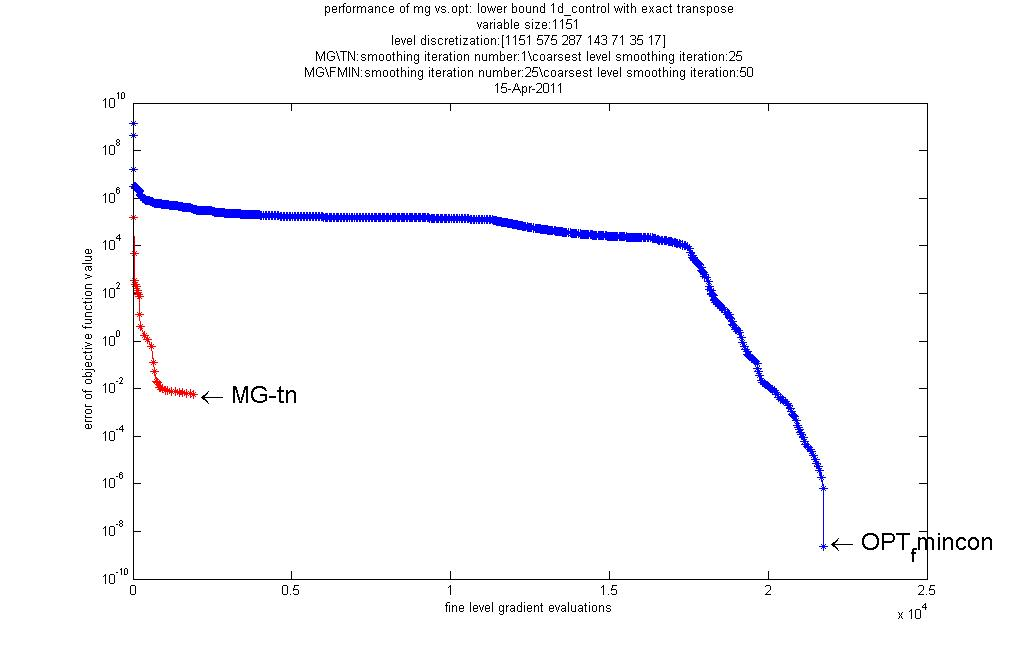
\includegraphics[width=1.0\textwidth]{plot_exact_tr_1sb1151.jpg}
  \caption{Test on Coarse approximation}
\label{fig:1s1151}
\end{figure}
\begin{itemize}
\item 1st approach tried to resolve this issue: Downdate the variable simply by injection rather than full weighting, in this way the convergence can be improved but still couldn't show obvious benefit than opt to completely converge
\item 2nd approach is to apply the bound constraint introduced in paper from Toint and will also sligly improve the convergence although it is still not quick enough.
\item 3rd approach is to fix the binding without moving in the line search of MG/OPT with $\alpha_{0}=1$. But no $\alpha$ can satisfy $f(x+\alpha p)< f(x)$ even though $e\tr Gvmg <0$
\end{itemize}
\item Question: The tests we did on our last meeting to compare the step to solution and search direction will become very different in only 3 cycles (actually comparing to step, search direction is too tiny) is  I modified the way to approximate the lagrangian multiplier $\lambda$ by simply pick the nonzero entries of $\lambda$ as the components of variables which are binding in 'sfun'. Instead, if I use the entries as 'ipivot' assigned from TN, then it will show more similarity between step to solution and search direction for all cycles until error of $10^{-2}$ magnitude. So what's the real difference between these two ways.
\end{itemize}    



\section{2-side bound constrained problem} 
\begin{itemize}
\item Objective problem:  \\

$min f(x)=\frac{1}{2}  x\tr Ax-b\tr x\, s.t.\, \{
\begin{array}  {rcr}
 1-x \leq 0\\
 x-5\leq 0\\
\end{array}$\\

\item Compare the original coarse solution with solution of shifted problem. The formula I used is to compare $v_{s}^{*}-\bar{v_{H}}$ with $v_{H}^{*}-\bar{v_{H}}$.
\begin{itemize}
\item Result: it turns out that this compare has the same shape plot as the comparing we did before which is  between the step to solution with search direction on the fine level. i.e. As applying more loop of MG/OPT, the search directions for both fine and coarse level become much more slight comparing to step to solution.
\item Conclustion: The coarse level approximation couldn't  give a enough step for fine level to converge, that's why MG/OPT on the fine level didn't make progress after few cycles. Motivatived by this fact, I found out that the primal reason for the stalling on fine level is because TN couldn't provide a positive step length $\alpha_{0}$ to update $\bar{v_{h}}$ based on the computation of $\alpha_{0}$ which is chosen as the minimum of feasible search direction $p$ get from Conjugate-Gradient. Thus, once the variable hits the bounds, $\alpha_{0}=0$ . Therefore, the progress for $\bar{v_{h}}$ can only be obtained from coarse level. i.e. $k_{1}=k_{2}=0$.
\begin{itemize}
\item Since $\IhH \IHh v_{H}\approx v_{H}$. In another word, the initial point for coarse shifted problem will be close to its solution and in turns bring a ting search direction with no moving on fine level.
\item Because of this reason,  I tried another approach for $\alpha_{0}$ that fix $\alpha_{0}=1$ and during the line search process, fix those binding points without moving to guarantee the feasibility, more progress can be obtained then. But couldn't completely converge yet due to the same issue happened for 1-side bound case about the full weighting downdate.
\end{itemize}  
\end{itemize}
\item  \footnote{\bf Note: All the tests have been done upon two different version of line search in TN: 
\begin{itemize}
\item 1st : $\alpha_{0}$ is chose as the minimum of feasible search direction $p$ get from Conjugate-Gradient
\item 2nd: Fix $\alpha_{0}=1$ and during the line search process, fix those binding points without moving to guarantee the feasibility
\end{itemize}
} Test if $\hat{v_{H}} \equiv \bar{v_{H}}+\IhH(v^{*}-\bar{v_{h}}) \approx v_{s}^{*}$ where $v_{s}^{*}$ denotes the solution of shifted coarse problem. 
\begin{itemize}
\item  Test problem discretization level: $ [257,128]$
\item TN line search:  tried both version of $\alpha_{0}$
\item When MG/OPT works well, then $$v^{*}-\bar{v_{h}}\approx e_{h}=\IHh e_{H}=\IHh(v_{H}^{+}-\bar{v_{H}})$$
$$\IhH(v^{*}-\bar{v_{h}})\approx \IhH \IHh e_{H}=\IhH \IHh(v_{H}^{+}-\bar{v_{H}})$$ Therefore	
$$v_{s}^{*}\approx \bar{v_{H}}+(\IhH \IHh)^{-1}\IhH(v^{*}-\bar{v_{h}})$$ or roughly
$$v_{s}^{*}\approx \bar{v_{H}}+\IhH(v^{*}-\bar{v_{h}})$$
\item Result: They perfectly match each other, so we can have the conclustion that coarse approximation is right, shown in Figure \ref{fig:shift}. From another view, the search direction from coarse grid will be very tiny.
\begin{figure}[h]
\centering
  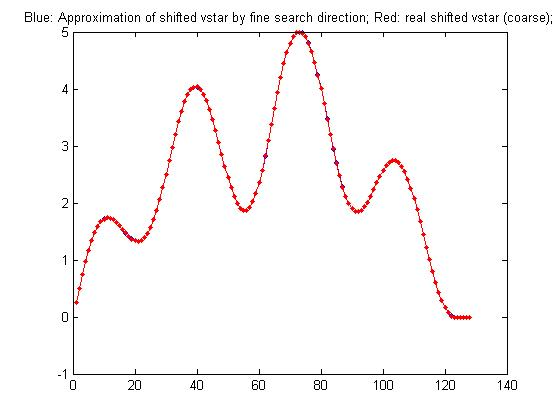
\includegraphics[width=1.0\textwidth]{shiftapprox.jpg}
  \caption{Test on Coarse approximation}
\label{fig:shift}
\end{figure}
\end{itemize}

\item I also tried MG/FMINCON on this problem, the convergence is stalled too, due to the fact of inner fmincon which will increase the function value even at all feasible point. I still need to understand more on this.

\item Then the next test is to treat constrained problem as unconstrained easily by setting $\hat{b}$ s.t.$f(x)=\frac{1}{2}  x\tr Ax-\hat{b}\tr x$ where $\hat{b}=b-\nabla c\tr \lambda$  with the known binding subscripts $\{i_{1},i_{2},\dots\}$. 
\begin{itemize}
\item test discretization level: $[17,8]$
\item The performance of MG/OPT is just as expected for unconstraint problem.
\end{itemize}

\end{itemize}




























\end{document}
